\part{Calculs acoustiques}
	\chapter*{Introduction}
	\addcontentsline{toc}{chapter}{Introduction}
Dans cette partie, nous allons traiter d'acoustique, d'algorithmes et de mathématiques. Chacune de ces disciplines permettra de répondre aux questions suivantes : Pourquoi ? Quoi ? Comment ? Voyons donc ces problématiques une par une.\\

\textit{\textbf{Pourquoi ?}} L'objectif de notre projet, maintenant que nous disposons d'une maquette virtuelle du théâtre d'Orange, est d'en étudier l'acoustique. Nous souhaitons pouvoir simuler, écouter et étudier le son qui était perçu dans ce lieu il y a deux mille ans. Outre le fait d'acquérir ces données, nous avons vu que les restitutions de certaines parties du théâtre était plus ou moins hypothétiques. Nous pourrons comparer ces différentes tentatives de restitution et en mesurer l'impact visuel mais également auditif. Les rares écrits antiques et les récentes études acoustiques sous-entendent que les Romains, et avant eux les Grecs, se basaient énormément sur la physique des matériaux et la géométrie des monuments pour optimiser la propagation sonore. Nous allons donc tenter d'apporter notre pierre à l'édifice au sujet de cette question. L'une de nos contraintes sera alors d'obtenir des résultats sur l'acoustique selon différentes géométries du bâtiment et divers matériaux. Il faudra également que le temps de calcul de chaque essai soit relativement court afin de pouvoir multiplier les configurations.

\textit{\textbf{Quoi ?}} Cet objectif nous a amené à développer un outil de calcul numérique répondant à des problématiques précises. Il complète ainsi la première partie de notre projet en s'interfaçant directement au logiciel Blender. Nous pourrons alors facilement étudier la maquette virtuelle du théâtre d'Orange précédemment présentée. Néanmoins, il est important de noter que cet outil est générique. Il pourra donc agir sur différents type de problèmes. Dans cette partie nous verrons quelle méthode de calcul a été retenue et les raisons qui ont poussé à faire ce choix. Effectivement, le théâtre d'Orange est un problème complexe car le maillage comporte plusieurs centaines de milliers d'éléments et sa géométrie peut inclure des surfaces concaves, convexes ou toutes sortes d'obstacles. Les outils présents sur le marché ont des limites par rapport à ce cas d'utilisation. Notamment, l'étude se portera aussi sur les résultats d'analyse. Comment visualiser des résultats acoustiques ? Peut-on, par une écoute d'un signal sonore, conclure des résultats ? Peut-on trouver des méthodes ergonomiques d'analyse ? Pour pouvoir répondre à ces questions, il est primordiale de disposer d'un accès total à la technologie. C'est pourquoi un outil complet a été développé pendant ce projet.

\textit{\textbf{Comment ?}} Tout code informatique présente une part de calcul, et qui dit calcul, sous-entend mathématiques. Ainsi, nous verrons les méthodes et astuces mathématiques qui ont permis de développer ce programme. Nous détaillerons les notions de lancer de rayons statistique, de sources images spatialisée et de réponse impulsionnelle. Aussi, nous verrons comment sont optimisées les performances par un procédé de "\textit{divide and conquer}" utilisant des octree. Un chapitre est également consacrer à la validation de l'algorithme en utilisant notamment des méthodes analytiques.\\

Pour débuter, nous ferons un tour d'horizon de la physique de l'acoustique et plus concrètement dans le cas qui nous concerne, de l'acoustique de salle. Nous présenterons les différentes méthodes permettant d'étudier les lois acoustiques et présenterons leurs limites. Nous détaillerons alors les principes physiques utilisés pour notre algorithme avant de passer à la présentation de son architecture et à sa validation. Cette partie présente l'outil dans son contexte général et l'application au théâtre d'Orange sera faite dans la partie suivante.


\chapter{Acoustique de salle}
		\citationChap{
			La musique, c'est 50\% d'un film.}
			{Georges Lucas}
		\minitoc
		\newpage
		
\section{Introduction à l'acoustique de salle}
L'acoustique de salle est une discipline à part entière qui consiste principalement à étudier la réverbération d'une pièce soumis à une onde sonore. Le principe de cette étude est le suivant : Il s'agit en général de placer une source sonore à l'intérieur d'une salle, fermée ou non, et de la faire rayonner dans toutes les directions. L'onde se propage alors jusqu'aux parois et subit un phénomène de diffusion. Il s'agit en réalité d'une combinaison de trois phénomènes : la réflexion, la réfraction et la diffraction. Par réfraction on entend la notion d'absorption suivant les lois de Descartes sur la propagation entre deux milieux (\cite{jouhaneau}). La diffraction quant à elle opère lorsque la longueur d'onde est proche de la taille de l'obstacle. En se plaçant en un point à l'intérieur de la salle, on pourra alors recevoir un signal sonore comme étant la somme d'un champ direct et d’un champ réverbéré. Le son direct provient directement de la source sans n'avoir touché aucune surface. Le son réverbéré se distingue en deux catégories : les premières réflexions dont l'ensemble forment la texture du son et le champ diffus qui peut être assimilé à une somme infinie d'ondes se propageant dans toutes les directions. 
On comprend alors que les principaux facteurs qui vont influer sur l'acoustique perçue dans une salle sont : la source sonore, le milieu de propagation et la nature des parois et des obstacles.

\begin{figureth}
%\begin{subfigureth}{0.3\textwidth}
%	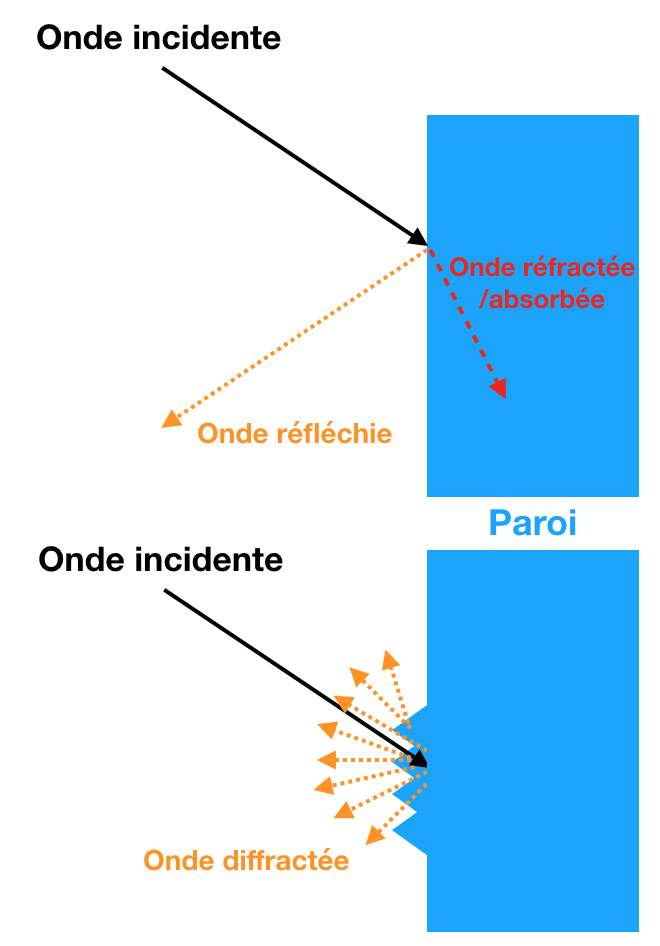
\includegraphics[width=\linewidth]{images/schema_absorption}
%	\caption{Schéma d'une onde en contact avec une paroi}
%	\label{schema_absorption}
%	\qquad
%\end{subfigureth}
%\begin{subfigureth}{0.65\textwidth}
	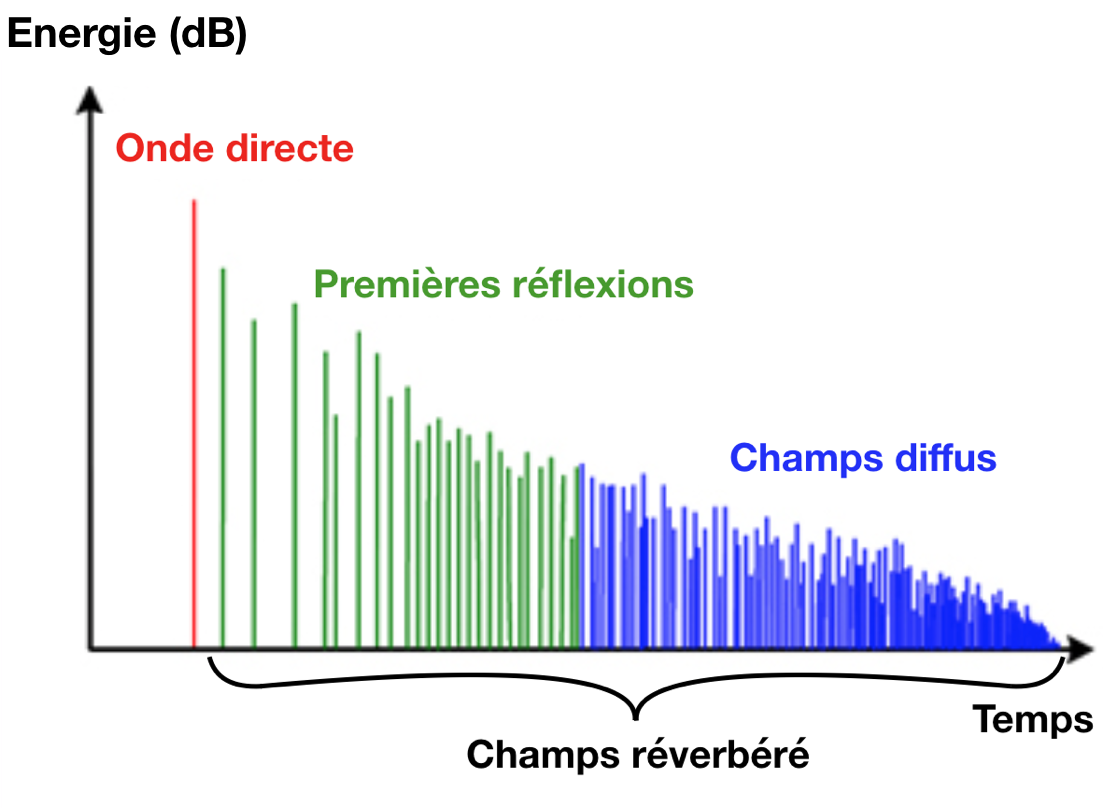
\includegraphics[width=\linewidth]{images/RIR_schematique}
	\caption{Réponse temporelle d'une impulsion sonore dans une salle}
	\label{RIR_schematique}
%	\end{subfigureth}
\end{figureth}

La figure \ref{RIR_schematique}, illustrant une réponse impulsionnelle, montre que l'information perçue est une succession d'ondes sonores arrivant décalées dans le temps. Si l'écart entre ces ondes est long, alors d'auditeur pourra les différencier et entendra le phénomène d'écho. Au contraire, si l'écart est suffisamment restreint et que les ondes sont mélangées au moment d'arriver à l'auditeur, alors celui-ci n'entendra qu'un son prolongé dont l'intensité diminue. Il s'agit de la réverbération (\cite[p. 39]{sabine}). 

\section{Méthodes de calcul acoustique} 
Le calcul de l'acoustique d'une salle peut se faire selon différentes méthodes. Nous allons succinctement en présenter quelques unes afin d'en dégagé les grands principes et les limites.

	\subsection{Principe statistique}

P. E. Sabine écrit en 1932 "\textit{Acoustics and architecture}" en reprenant les principes son homonyme W. Sabine. Ce dernier décrivait 20 ans plus tôt des protocoles de test pour mesurer des
temps de réverbérations dans les salle. P. E. Sabine considère que la réverbération suit un modèle purement statistique. De son point de vue, la densité d'échos à prendre en compte est suffisamment importante pour considérer le phénomène comme pseudo-aléatoire. \cite[p. 19]{Kandelman}. Il suppose ainsi que l’énergie sonore et le temps de réverbération sont uniformes en tout point de la salle. Ces considérations permettent d'exprimer ces deux valeurs l'une par rapport à l'autre comme par exemple dans la formule dite "de Sabine" : 

\begin{equation}
   	T = \frac{k.V}{A}
\end{equation}

Avec : \\
$k \approx 0,163$ \\
$V$ : le volume de la salle\\
et
\begin{equation}
   	A = \sum_{i=1}^N S_{i}\alpha_{i} + 4mV
\end{equation}
où : \\
$\alpha$ est le coefficient d'absorption \\
$m$ est l'amortissement du milieu (par exemple l'air) \\
$S_{i}$ est la surface de la i\up{e} \\
$N$ est le nombre de paroi total \\

La théorie de Sabine, est encore aujourd'hui couramment employée par les acousticiens des salles. Pourtant, cette hypothèse dite de "champ diffus" n’est plus vérifiée en pratique, dès lors que la forme du milieu de propagation n’est plus homogène et que l’absorption acoustique devient importante et non uniforme. De plus, cette théorie s’applique mal aux géométries présentant des ouvertures et, en particulier, dans le théâtre d'Orange. \cite[p. 60]{picaut}.

 
	\subsection{Méthode de résolution exacte}

La méthode de résolution exacte utilise le principe des éléments finis ou des éléments aux frontières. Il s'agit de mailler le domaine d'étude par des petits éléments linéiques (2D) ou surfaciques (3D). Sur chacun de ces éléments, on pourra calculer la pression acoustique par résolution de l'équation d'onde (modèle de Green ou Helmotz-Kirchhoff) en considérant les conditions aux limites. Cependant, même si l'implémentation mathématique ne présente pas de difficulté majeure, le problème se complique nettement selon la géométrie de la salle. Effectivement, la taille et donc le nombre d'éléments, dépendra de la longueur d'onde \cite[p. 740]{beamtracing}. Dans un cas comme le théâtre d'Orange où les longueurs se comptent en dizaines de mètres et les fréquences en kilo-Hertz (fréquences audibles), il faudra des mailles de l'ordre du millimètre, et donc des milliard d'éléments. Ce genre de problème est aujourd'hui quasi-impossible à mettre en place de part la puissance de calcul et l'espace mémoire nécessaire. Par ailleurs la création du maillage conforme de ce type représente une difficulté à part entière.
Au début du projet, nous avons tenté d'analyser une version très simplifiée du théâtre à des fréquences très faibles. Nous voulions notamment tester l'impact de la forme incurvée des gradins en comparant de manière récursive différents maillages. Le remaillage était effectué à l'aide de l'outil "\textit{mmg}" développé à l'\gls{iscd}. Les calculs acoustiques ont été effectués avec l'outil "\textit{MyBEM}" développé par le \gls{cmap}. En conservant à peu près des dimension du théâtre, nous obtenions plusieurs centaines de milliers d'éléments et des temps de calcul déjà de quelques dizaines de minute avec un ordinateur standard. Le constat a alors été que ce type d'étude serait trop complexe et les résultats difficiles à interpréter.

\begin{figureth}
	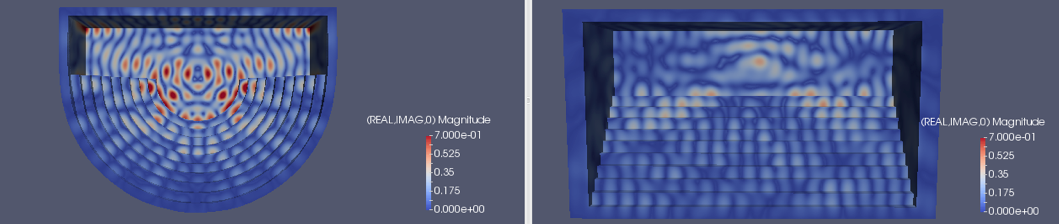
\includegraphics[width=\linewidth]{images/BEM}
	\caption{Comparaison d'un théâtre simplifié avec gradins coniques ou gradins cubiques par \gls{bem} à 50Hz}
	\label{BEM}
\end{figureth}

Explorons maintenant les méthodes approchées de type géométrique.

	\subsection{Méthode de tracé de rayon}
Tout d'abord, la méthode dite de tracé de rayon (\textit{ray-tracing}) qui est très souvent utilisée dans les logiciels d'acoustique de salle. Cette approche suppose que l’énergie sonore émise depuis une source est repartie sur un certain nombre de rayons rectilignes déviés de manière spéculaire lors de leur rencontre avec les parois. L'énergie d'un rayon sera atténuée selon le coefficient d'absorption des parois lors du rebond et décroitra comme la distance de propagation au carré afin de simuler l'effet de dispersion géométrique d'une onde sphérique. La mesure d'énergie est alors réalisée par comptage du nombre de rayons qui traversent le récepteur. La précision de mesure sera ainsi fonction du nombre de rayons émis et de la taille du récepteur. Il peut notamment y avoir beaucoup de perte d'information si le domaine de propagation est complexe \cite[p. 60]{picaut}. Il s'agit donc d'une méthode très puissante pour simuler les réflexions géométriques sur les paroi mais qui devient compliqué pour simuler les effets de diffraction. C'est aussi la seule méthode géométrique permettant de simuler des réflexions sur des parois courbes \cite[p. 13]{Kandelman}.

	\subsection{Méthode de lancé de particules}
Le lancé de particules est très similaire au tracé de rayon. Cependant, dans le concept des particules sonores, chaque particule est porteuse d’une énergie constante qui ne décroit donc pas comme la distance au carré. Lors du contact avec une paroi, la particule sera réfléchie de manière statistique. Par exemple, si $\alpha$ est le coefficient d'absorption de la paroi, alors, la particule aura une probabilité de $(1-\alpha)$ d'être réfléchie et une probabilité $\alpha$ d'être absorbée. En ce sens, il est alors également possible de déterminer, selon une loi de probabilité, l'angle de réflexion et simuler ainsi une "pseudo-diffusion" des matériaux. \cite[p. 62]{picaut}.
	
	\subsection{Méthode des sources-image}
Cette méthode est fondée sur la construction de sources virtuelles, images de la source réelle, construite par symétrie par rapport aux parois de l'enceinte. La contribution énergétique de chaque source-image est celle habituellement rencontrée dans le cas de la propagation en champ libre, pondérée par le coefficient d’absorption des parois considérées \cite[p. 60]{picaut}.
Le problème de cette méthode est que l'on génère l'ensemble des sources-images d'une salle et qu'il est ensuite difficile de discriminer celles qui sont perçues et celles qui sont bloquées par des obstacles. Cela est donc plutôt adapté aux pièce de forme concave et vide. Par ailleurs, comme pour le tracé de rayon, les effets de diffraction ne sont pas pris en compte. 

	
	
\section{Méthode couplée}

"\textit{Il faut également signaler que la plupart de ces approches, comme celles fondées sur les sources images et le tracé de rayons sonores, prennent difficilement en compte les effets météorologiques tels que le vent, les gradients de célérité du son et la turbulence atmosphérique, pourtant très importants en milieu ouvert}" \cite[p. 60]{picaut}.

Nous comprenons qu'aucune de ces méthodes pourrait convenir parfaitement à notre problème du théâtre d'Orange. Nous optons donc pour une combinaison des différentes approches géométriques ainsi que la théorie statistique évoquées précédemment. Avant de détailler le principe de la méthode utilisé, il est bon de rappeler certains principes physiques.

\begin{figureth}
\begin{subfigureth}{0.55\textwidth}
	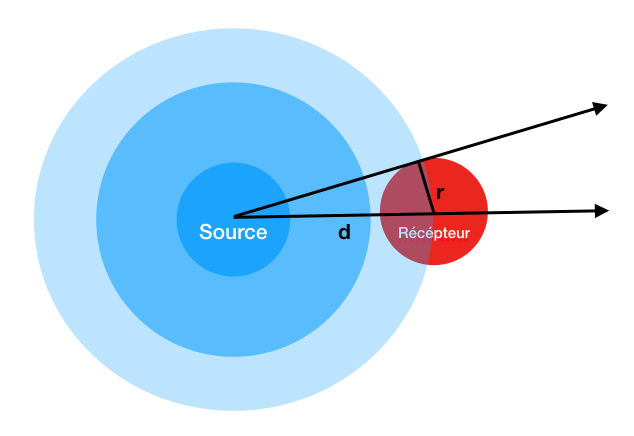
\includegraphics[width=\linewidth]{images/schema_propagation}
	\caption{Schéma en deux dimensions d'une onde sphérique dont une portion d'énergie est mesuré par un récepteur de rayon r.}
	\label{schema_propagation}
\end{subfigureth}
\qquad
\begin{subfigureth}{0.35\textwidth}
	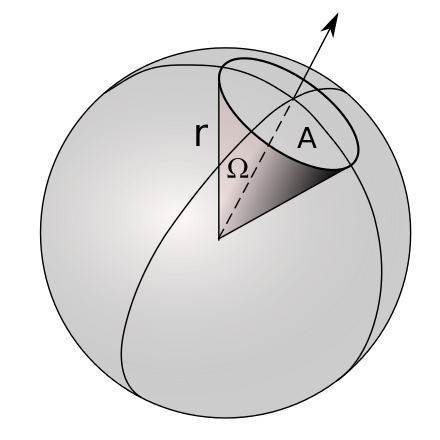
\includegraphics[width=\linewidth]{images/angle_solide}
	\caption{Représentation de l'angle solide d'un cône de révolution \footnotemark}
	\label{angle_solide}
	\end{subfigureth}
\end{figureth}
\citefnt[image]{angle_solide}

Nous nous plaçons dans le cas d'une source impulsionnelle. Effectivement, un signal sonore continu peut-être discretisé par une suite d'impulsions. C'est d'ailleurs le cas de tout signal numérique qui est échantillonné à une certaine fréquence. Nous prenons également le cas, le plus courant, d'une source omnidirectionnelle qui émet de l'énergie de manière uniforme dans toutes les directions de l'espace. Une impulsion étant un signal d'un temps infiniment court, l'énergie émise depuis la source sera répartie sur la surface d'une sphère en expansion. Si l'on mesure à différents instants une portion de taille constante de la sphère, on obtient une valeur inversement proportionnelle au carré de la distance. En d'autres mots, on considère que l'énergie mesurée est l'intersection entre un récepteur de forme sphérique, de rayon $r$, constant et de la sphère supportant l'énergie totale. Ainsi, si on considère que :

\begin{center}
   	$E_{tot} \propto S_{tot}$\\
	et $E_m \propto S_m$
\end{center}

Avec	: \\
$E_{tot}$ l'énergie totale \\
$S_{tot}$ la surface de la sphère portant l'énergie \\
$E_m$ l'énergie mesurée \\
$S_m$ la surface de la sphère de mesure \\
\\
Alors :
\begin{center}
   	$E_{tot} \propto d^2$\\
	et $S_m$ est constante\\
\end{center}

Donc :
\begin{equation}
	E_m \propto \frac{E_{tot}}{d^2} \propto \frac{1}{d^2}
\end{equation}


Il s'agit de la loi de propagation géométrique d'une onde sphérique qui comporte donc une énergie à décroissance quadratique. Cette propriété physique devra apparaitre dans le résultat final.

Par ailleurs, nous choisissons une approche discrète. Non pas dans le sens de ne pas être repéré par nos ennemis, mais plutôt dans celui d'une discrétisation de l'énergie surfacique. La source sonore ne va donc pas émettre une sphère mais va plutôt projeter de manière uniforme un nombre de $N$ de rayons. Chacun porte l'énergie $\frac{E_{tot}}{N}$. Cependant, comme nous l'avons vu précédemment, l'approximation discrète apporte de l'erreur au résultat car l'information n'est présente qu'au niveau des rayons et non dans l'espace entre deux. C'est pourquoi nous allons chercher à limiter cette erreur. Pour cela, nous devons exprimer le temps au bout duquel il est possible de capter moins d'un rayon dans la sphère de mesure. L'analyse étant théorique, nous effectuons ce raisonnement en espace libre. 

\begin{figureth}
	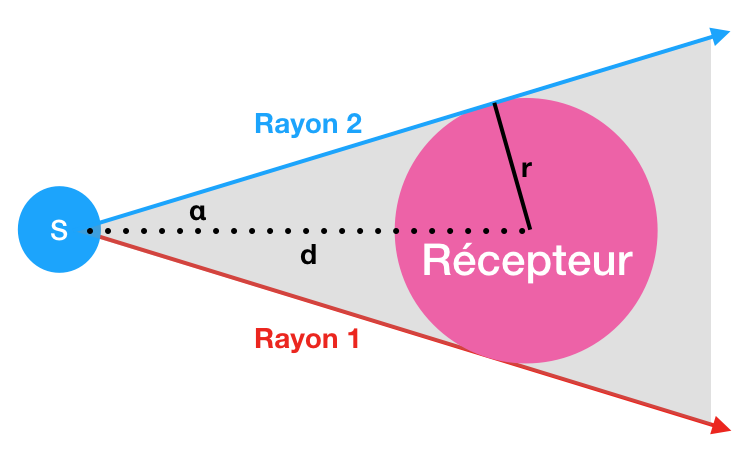
\includegraphics[width=0.8\linewidth]{images/schema_rayon}
	\caption{Schéma d'un récepteur captant au moins un rayon.}
	\label{schema_rayon}
\end{figureth}

Pour cela, nous utilisons la formule de l'angle solide d'une cône :
\begin{equation}
	\Omega = 2\pi(1-cos(\alpha))
\end{equation}

Nous avons vu précédemment que cet angle solide pouvait aussi s'exprimer :
\begin{equation}
	\Omega = \frac{E_{tot}}{N}
\end{equation}

Pour : \\
$r$ : le rayon du récepteur \\
$d$ : la distance maximale du récepteur à la source \\
$N$ : le nombre de rayons total \\

Alors, d'après Pythagore (voir fig. \ref{schema_rayon}) :
\begin{align}
	cos(\alpha) & =  \frac{\sqrt{d^2-r^2}}{d}  \\
	& =  \sqrt{1-\frac{r^2}{d^2}} \\
	& \simeq 1-\frac{1}{2}\frac{r^2}{d^2}
\end{align}

Car on suppose que le rayon de mesure $r$ sera petit devant la distance $d$ parcourue par l'onde. On a alors :

\begin{align} 
	& 2\pi(1-(1-\frac{1}{2}\frac{r^2}{d^2})) = \frac{4\pi.d^2}{N} \\
	\Rightarrow & \qquad d^2 = \frac{r}{2}\sqrt{N} \label{seuil_arret}
\end{align}

Nous constatons alors que nous pourrons fixer $N$, le nombre de rayons d'énergie total émis depuis la source et $r$, le rayon de la sphère de mesure, pour connaitre la distance $d$ au bout de laquel la probabilité de ne capter aucun rayon sera non nulle. En pratique, on voudra réduire encore l'erreur et il faudra arrêter la mesure avant d'arriver à cet extreme. On pourra alors fixer un nombre $n$ de rayons minimum à capter. Par exemple si on fixe $n$ à 100 rayons, on s'assure que la mesure comprend au moins 100 portions de la sphère énergie et on revient statistiquement à un modèle quasi-continu.

Pour établir la nouvelle expression, il suffit de refaire les mêmes calculs en considérant que :
\begin{equation}
	\Omega = n.\frac{E_{tot}}{N}
\end{equation}

L'équation \ref{seuil_arret} s'écrit donc :
\begin{align} 
d^2 = \frac{r}{2}\sqrt{\frac{N}{n}}
\end{align}

Nous obtiendrons de cette façon les premières réflexions de la réponse impulsionnelle. Cependant, les réponses impulsionnelles acoustiques sont en général calculées jusqu'à ce que l'énergie diminue de $60dB$. Il s'agit d'un critère d'arrêt classique de car il assure de couvrir la plage d'audition humaine. Or avec notre méthode, nous ne prenons plus de mesure à partir d'un certain temps, correspondant à la distance $d$. Il faudra alors jouer sur les paramètres $N$, $r$ ou $n$ pour s'assurer de dépasser le \gls{RT60}. En pratique, le temps de calcul sera très sensible à ces paramètres et il sera plus judicieux d'arrêter la mesure avant. On pourra alors compléter le champs diffus de manière statistique d'après les hypothèses de Sabine. La réponse impulsionnelle sera prolongée par régression linéaire pour atteindre \gls{RT60}.


Le principe de la méthode utilisée consiste donc à propager des rayons à partir d'une source et d'analyser ceux qui traverseront une sphère-récepteur. Leur temps de parcours permet de créer la \gls{rir}. Celle-ci pourra alors être convoluée à un signal audio pour créer un son réverbéré. Le chemin de chacun de ces rayons permet aussi de situer dans l'espace la source-image correspondant, c'est à dire l'image de la source suite aux divers réflexions sur les parois (voir fig. \ref{schema_SI}. Nous obtenons ainsi une constellation de sources-images portant les énergies associées à leurs rayons. Cela permettra par la suite de spatialiser le son. Il sera alors possible de connaître la provenance des échos et ainsi d'écouter le son réverbéré en trois dimensions.

\begin{figureth}
	\begin{subfigureth}{0.45\textwidth}
		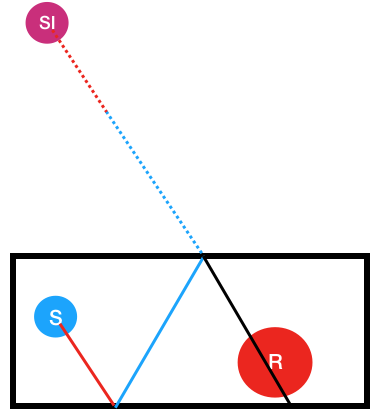
\includegraphics[width=0.8\linewidth]{images/schema_SI}
		\caption{Schéma de la création d'une source image par réflexions successives d'un rayon sur les parois d'une salle}
		\label{schema_SI}
	\end{subfigureth}
	\qquad
	\begin{subfigureth}{0.45\textwidth}
		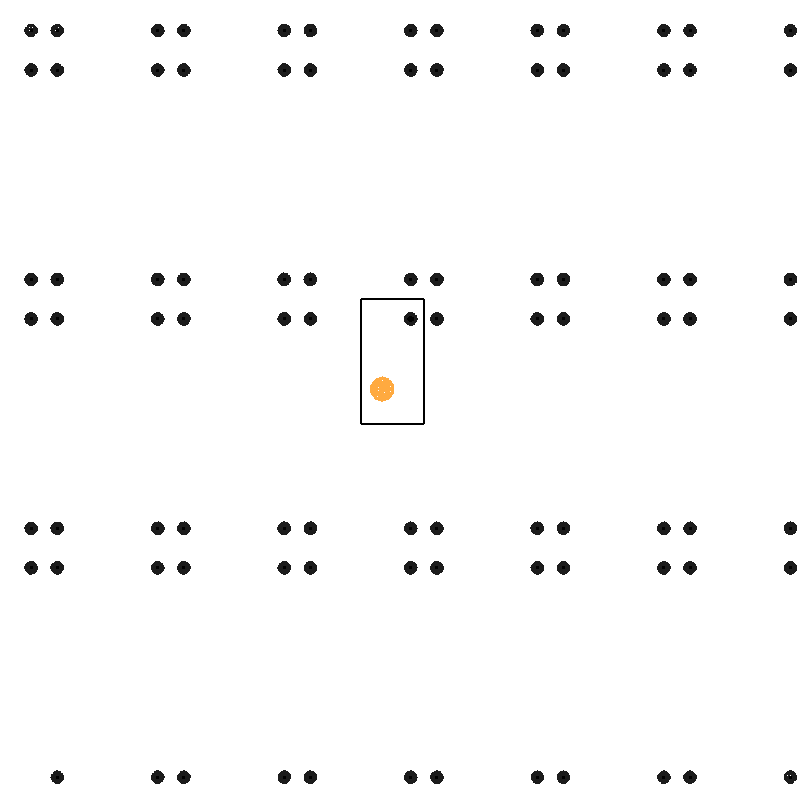
\includegraphics[width=0.8\linewidth]{images/constellation}
		\caption{Constellation de sources-images dans une salle rectangulaire}
		\label{constellation}
	\end{subfigureth}
\end{figureth}
		
\chapter{Logiciel développé}
	\citationChap{
	Quand on aime on ne compte pas... \\
	Ça tombe bien, je suis mauvaise en calcul !
	}{Sophie Lesellier}
	\minitoc
	\newpage
	
\section{Introduction}
Le projet a pour essence le calcul de l'acoustique du théâtre d'Orange. Cela soulève certaines problématiques qui nous ont poussé à développer un nouvel outil de calcul acoustique. Ce travail à été initié pour pouvoir répondre au cahier des charges suivant :
\begin{itemize}
	\item Permettre l'étude acoustique d'un bâtiment.
	\item Permettre la modification rapide de la géométrie du maillage et des matériaux.
	\item Avoir un total contrôle de la technologie afin d'en connaitre précisément le fonctionnement et d'accéder aux données brutes.
	\item S'interfacer facilement avec Blender.
	\item Calculer les résultats sur une large plage de fréquences audibles (50-8000Hz).
	\item Prendre en compte l'absorption atmosphérique.
	\item Pouvoir utiliser des maillages non conforme avec divers niveaux de raffinement et plusieurs centaines de milliers d'éléments.
	\item Avoir un temps de calcul faible pour pouvoir multiplier les tests.
	\item Disposer de résultats numériques non ambiguës ainsi que de résultats visuels et auditifs.
\end{itemize}

Afin de répondre à ces contraintes, nous avons opté pour certains choix technologiques. Premièrement, le code est développé en C++ pour des raisons de rapidité de calcul. Il s'agit d'un exécutable "client" paramètrable directement depuis l'interface Blender. Au lancement du programme, Blender exporte le maillage dans un fichier qui sera traité par le logiciel "client". Ainsi, l'outil acoustique est transparent pour l'utilisateur et l'accès au maillage est donc immédiat. Le format de fichier s'est porté sur le \gls{obj}. Celui-ci est un des formats les plus courants et disponible sur la plupart des logiciels de \gls{cao}.Ainsi, l'outil n'est pas exclusif et pourra travailler à partir de n'importe quel maillage au format \gls{obj}.

Nous choisissons dans un premier temps d'utiliser des sources omnidirectionelles, c'est à dire qui propage le son de manière uniforme dans toutes les directions de l'espace. C'est avec ce principe que nous décrirons l'algorithme. Notons par contre qu'il serait possible d'utiliser d'autre types de source en changeant la répartitions des rayons émis. De même nous ne traiterons pas l'aspect de diffraction des parois. Comme nous l'avons évoqué précédemment, il est possible d'utiliser des lois de probabilité sur la direction de réflexion des parois. Nous choisissons néanmoins de ne fonctionner qu'avec des réflexions spéculaires car le sujet de la diffraction est extrêmement vaste et complexe. Il s'agit d'un sujet à part entière que l'on ne traitera pas durant ce projet.

La figure \ref{synopsis} présente de manière synthétique l'architecture logicielle développée au cours du projet. Cette partie présentera en détails les différentes briques de l'outil de calcul acoustique. Nous présenterons d'abord la partie algorithmique conçue en C++ et finirons par la l'interface homme-machine accessible depuis Blender.

\begin{figureth}
	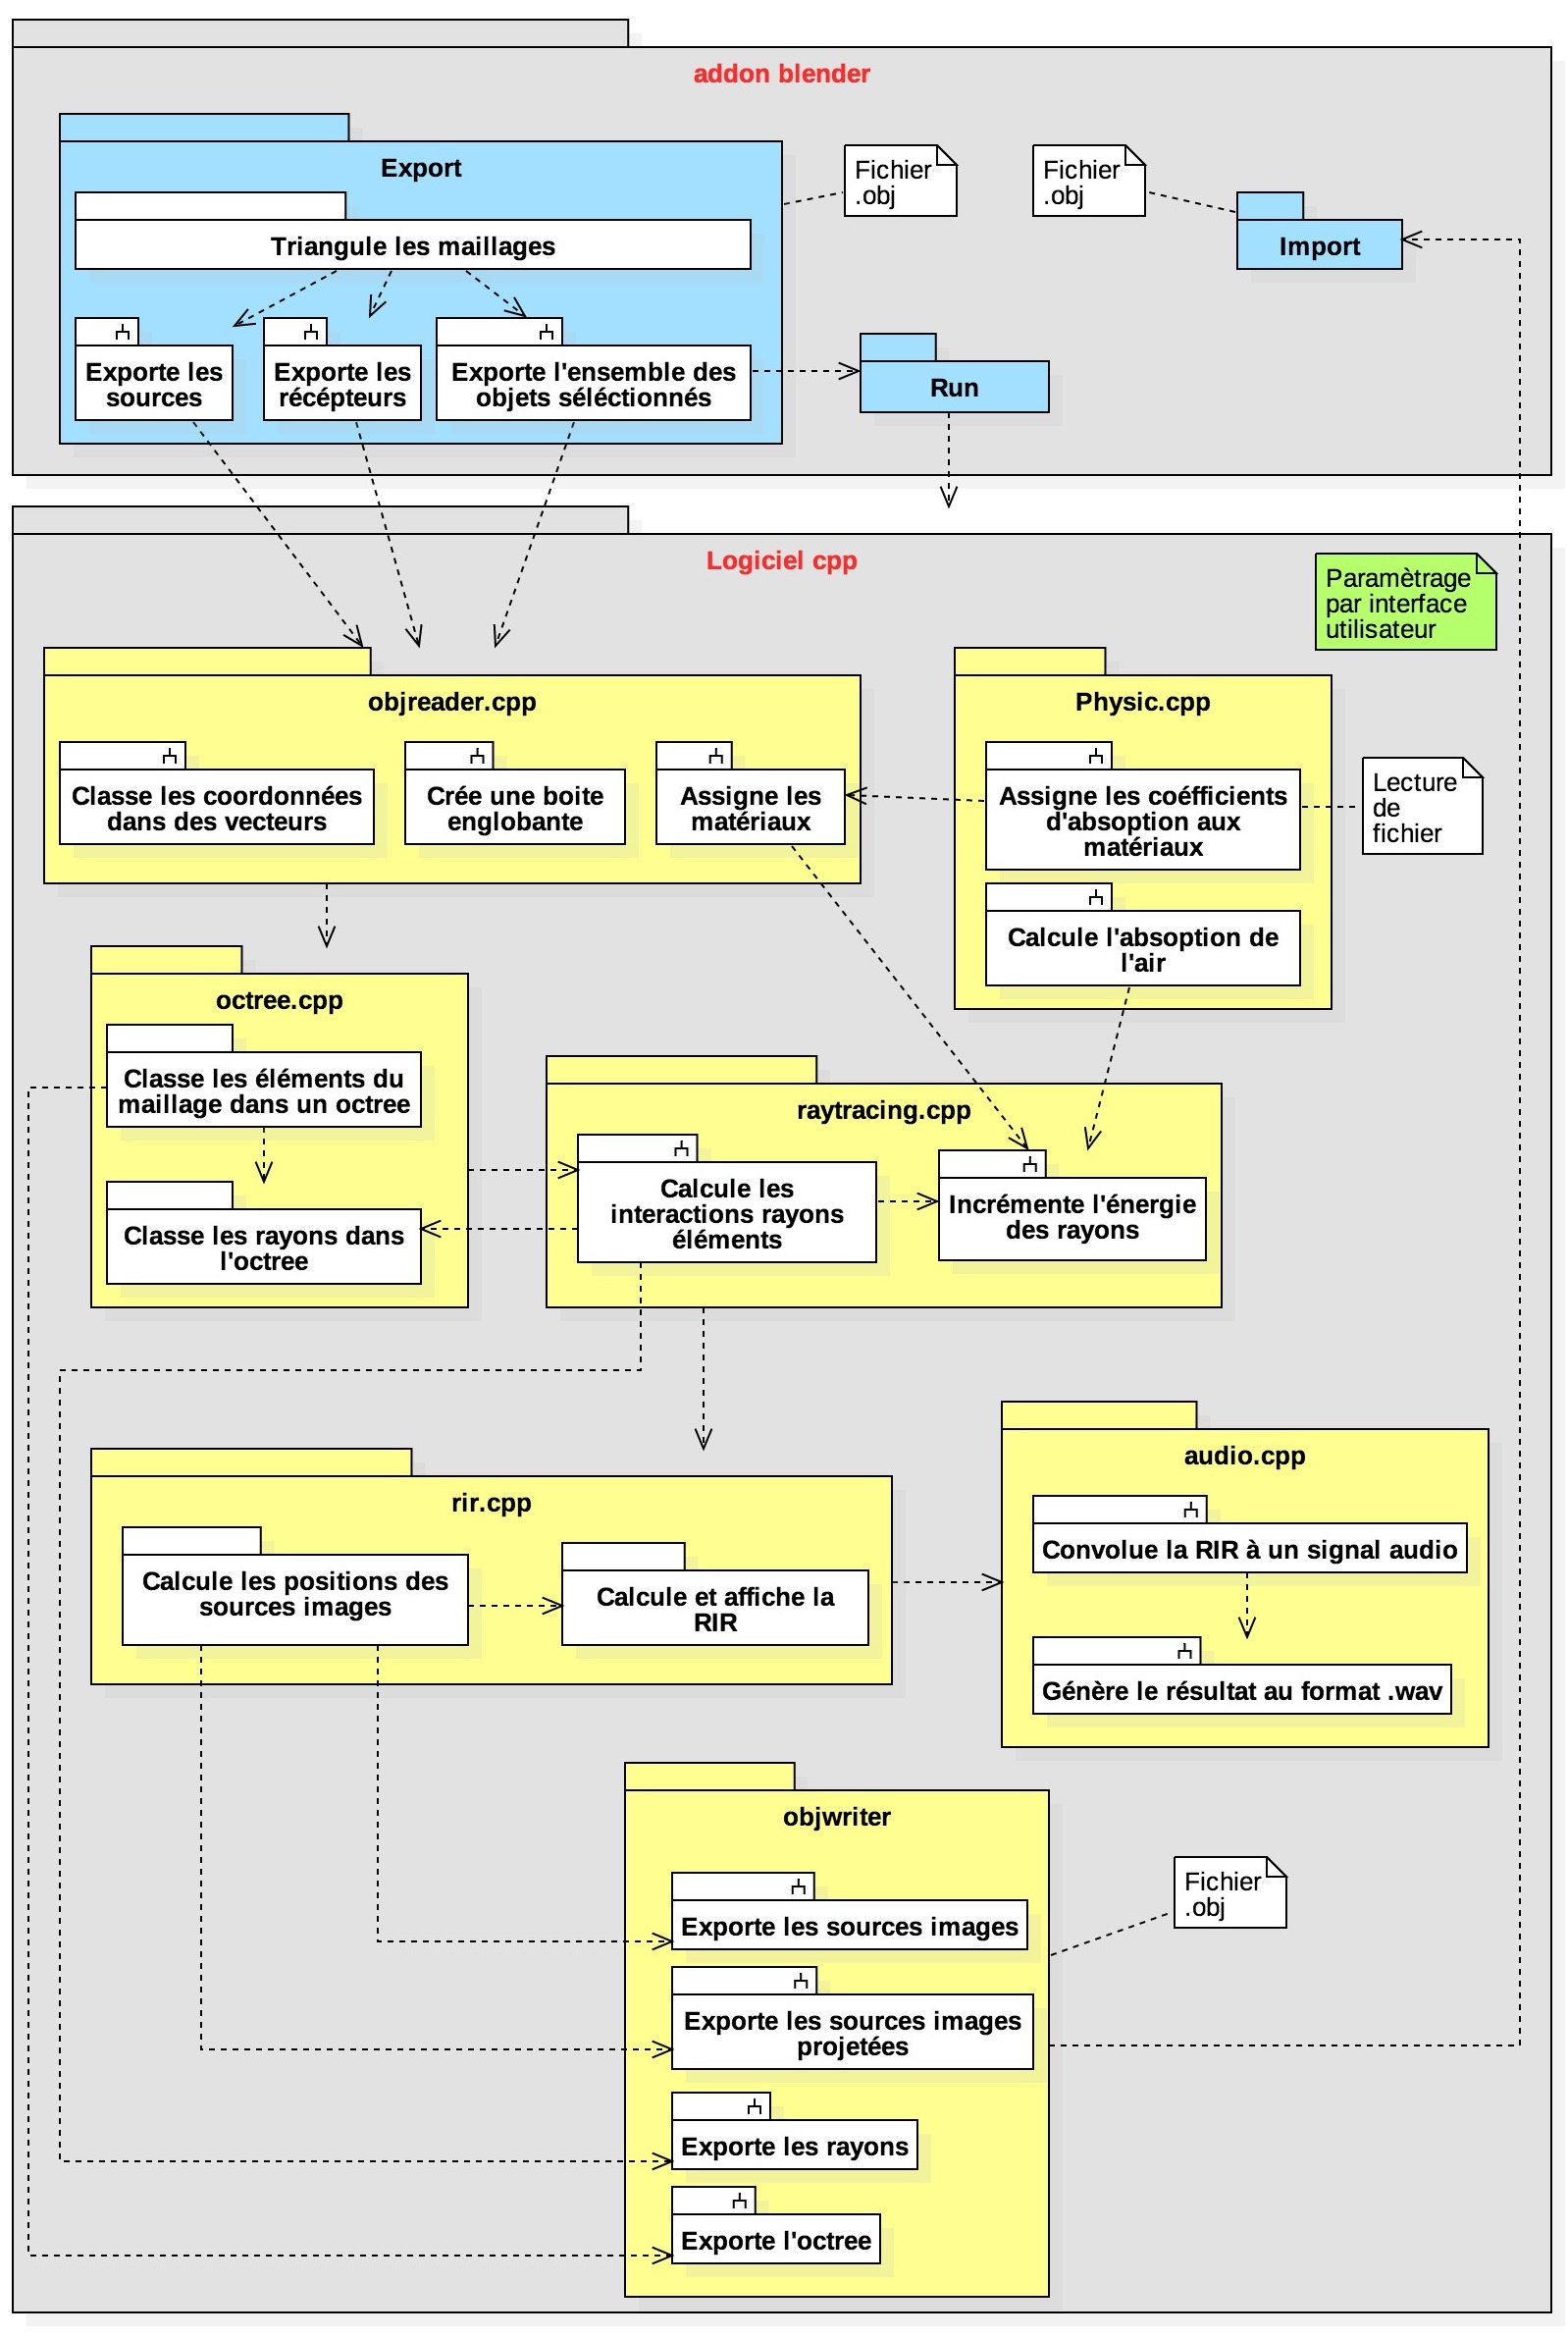
\includegraphics[width=\linewidth]{images/synopsis}
	\caption{Synopsis de l'architecture logiciel développé pour le calcul d'acoustique de salle}
	\label{synopsis}
\end{figureth}


\section{Initialisation}
Au démarrage du logiciel, avant de lancer le calcul acoustique, plusieurs paramètres s'initialisent.

\subsection{Lecture des matériaux}
L'une des premières étape consiste à lire une base de donnée de matériaux (issue du logiciel Odéon) et d'associer leur référence à leur huit coefficients d'absorption. La référence est un nombre qui pourra être stipulé dans le nom du matériau sous Blender. Celles-ci sont associées dans la base de donnée à huit coefficients d'absorption correspondant aux bandes d'octave : 62,5Hz, 125Hz, 250Hz, 500Hz, 1kHz, 2kHz, 4kHz, 8kHz. Ces huit bandes de fréquence permettent de couvrir une large plage des fréquences audibles par l'être humain. Il existe de nombreuses bases de données recensant ces coefficients d'absorption pour tout type de matériaux. Elles sont en générales créées de manière expérimentale et celle que nous utilisons a l'avantage d'être très complète et en libre accès sur le site d'Odéon \cite[Materials]{odeon}

Voici quelques exemple de coefficients d'absorption :
\begin{tableth}
\footnotesize
	\begin{tabular}{| c | m{2.5cm} | *{8}{c|}}
		\hline
		Référence & Nom du matériau & 62,5Hz & 125Hz & 250Hz & 500Hz & 1kHz & 2kHz & 4kHz & 8kHz \\
		  \hline
		  \hline
		   1 & 100\% absorbent & 1 & 1 & 1 & 1 & 1 & 1 & 1 & 1 \\
		   \hline
		2 & 100\%reflecting & 0 & 0 & 0 & 0 & 0 & 0 & 0 & 0 \\
		   \hline
		107 & Concrete block, coarse\footnotemark & 0.36 & 0.36 & 0.44 & 0.31 & 0.29 & 0.39 & 0.25 & 0.25 \\
		   \hline
		3000 & Hollow wooden podium\footnotemark & 0.4 & 0.4 & 0.3 & 0.2 & 0.17 & 0.15 & 0.1 & 0.1 \\
	     \hline
	 \end{tabular}
	\caption{Exemples de coefficients d'absorption de la base de donnée Odéon}
	\label{exempleOdeon}
\end{tableth}
\footnotetext{Harris, 1991}
\footnotetext{Dalenbäck, CATT}


\subsection{Lecture de maillage}
Comme évoqué précédemment, l'outil traite les données à partir d'un fichier \gls{obj}. Pour faciliter la lecture du maillages, on s'assurera de n'avoir que des faces triangulaires.  permet cela et cette Cela est réalisé automatiquement lors de l'exportation du fichier par un \gls{modifier} "triangulate" inclue dans le script d'export. Dans fichier de maillage, chaque objet est différencié par un en-tête comprenant son nom. S'en suit les coordonnées de l'ensemble de ses sommets (ou vertices), de ses textures et de ses normales. Ensuite sont regroupées par matériaux, les faces par combinaison de trois vertices, d'une texture et d'une normale. Les données sont transformées en un vecteur de coordonnées des sommets et un vecteur de coordonnées des normales. Les textures ne nous sont pas utile. Les coefficients d'absorption des matériaux sont aussi assemblés dans un vecteur en les classant dans le même ordre que les normales.
Les sources et récepteurs sont positionnés dans Blender. Il suffit d'utiliser les objets volumiques et que leur nom comporte respectivement "source" et "listener". L'outil de calcul déterminera alors le centre des objets sources et récepteurs en calculant la moyenne des coordonnées des sommets ainsi que le rayon du récepteur grâce à la distance entre son centre et une extrémité.

\subsection{Création d'une boite englobante}


\subsection{Calcul de l'absorption de l'air}


\section{Méthode d'octree}
\section{Calcul de rayon}
\section{Calcul de sources-images}
\section{Génération de réponse impulsionnelle}
\section{Vue d'ensemble}
Add-on blender, traitement du signal, etc

\chapter{Validation}
	\citationChap{
	L'observateur modifie ce qu'il observe. Certains événements ne se produisent que parce qu'ils sont observés. Sans personne pour les voir ils n'existeraient pas. 
	}{Bernard Werber}
	\minitoc
	\newpage
	\section{Introduction}
	Rappel cahier des charges
	\section{Comparaison aux cas test}
		\subsection{Salle rectangulaire}
		\subsection{Salle sphèrique}
	\section{Analyse de complexité}
	
\chapter*{Conclusion}
\addcontentsline{toc}{chapter}{Conclusion}
	\newpage
	
% Biblio
 \bibliographystyle{francaissc}
 \bibliography{Part2/Biblio}
\addcontentsline{toc}{chapter}{Références}
